%++++++++++++++++++++++++++++++++++++++++
% Don't modify this section unless you know what you're doing!
\documentclass[letterpaper,12pt]{article}
\usepackage{tabularx} % extra features for tabular environment
\usepackage{amsmath}  % improve math presentation
\usepackage{graphicx} % takes care of graphic including machinery
\usepackage[margin=1in,letterpaper]{geometry} % decreases margins
\usepackage{cite} % takes care of citations
\usepackage[final]{hyperref} % adds hyper links inside the generated pdf file
\hypersetup{
	colorlinks=true,       % false: boxed links; true: colored links
	linkcolor=blue,        % color of internal links
	citecolor=blue,        % color of links to bibliography
	filecolor=magenta,     % color of file links
	urlcolor=blue         
}
\usepackage{setspace,caption}
\usepackage{lipsum}
\captionsetup{font=doublespacing}% Double-spaced float captions
\doublespacing% Double-spaced document text
\usepackage{mathtools}
\usepackage{cuted}
%++++++++++++++++++++++++++++++++++++++++


\begin{document}
\title{Introduction of First Principle Calculation}
\author{Yan Sun}
\date{}
\maketitle

\begin{abstract}
The development of computation technology brings a significant acceleration to the scientific research. Nowadays, physics theory could be combined with the computation technology, simulating the behavior of particles and thus extracting the desired calculated data. First principle calculation is one of the most important calculation methods that initializes the computation based on the electron behaviors of systems, which is able to obtain results reach high level of accuracy compared to results of virtual experiment and has attracted much attention.  Both the development of theory and publicized coding project is contributing to make this calculation method more helpful to the scientific research.
\end{abstract}

\section{Introduction}
\par Traditional research approach is the combination of theoretical research and corresponded experiment results. However, this traditional research approach could be problematic. First, the experiment could be time-consuming and with low-efficient. For instance, the process to find a optimum ratio of composition for specific materials always obey the try-error process. This process means researchers usually need to do the experiments with multiple combinations of possible composition and then obtain the result. If the result is not reasonable another time of repeated work for different compositions should be tried again, which always take a lot of time. Second, the traditional method is always hard to analyze the electronic level or atomic level internal mechanism directly. Many auxiliary characterization approach will always be utilized to make support for the explanation of the obtained behaviors. The behaviors of particles mostly could be analyzed by the mathematical derivation but there are often many particles in the object system so it is unfeasible to do the analysis just by the manually calculation.\\
\par With the development of computation technique, especially the advanced hardware and parallel computing technique, large amount of calculation could be finished within very short time. These new technology could also make the research related calculation extremely fast, which initializes the computational research approach\cite{lee2016computational}. Nowadays, the computational part could be effective and efficient research method. Combined with theoretical derivation and the comparison with experimental results, it could help obtain massively results efficiently and even gives the prediction for the results under extreme environment that is difficult to reach. What's more, it could be applied to different particle scale, which could make computational research applied to many research fields and engineering fields, specifically showed in Figure \ref{scales}.

\begin{figure}[ht]
\centering
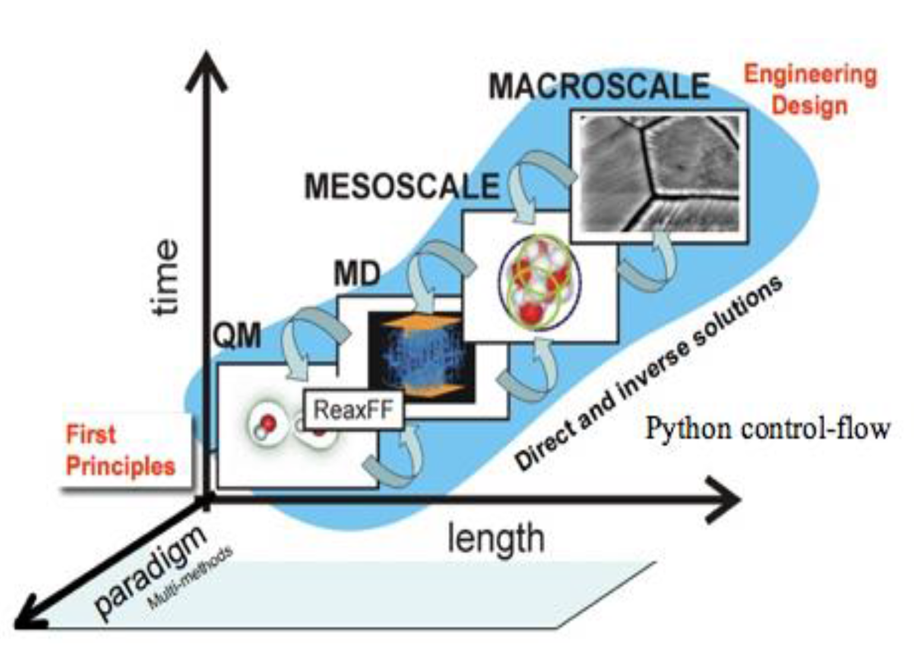
\includegraphics[width=0.5\textwidth]{./images/DifferentScales}
\caption{\label{scales}Computation for different scales\cite{luintroduction}}
\end{figure}

\section{First Principle Calculation Theory}

\subsection{Basic Approach}

First principle calculation is based on the quantum mechanics theory and condensed matter physics. During the calculation process, the most important target is to solve Schr\"{o}dinger Equation (Equation \ref{schrodinger}). Once the equations are solved, the wave functions, eigenfunctions and eigenvalues could be know. Then the energy of the system could also be obtained, which could be the basis of extracting more physical properties. 

\begin{equation} \label{schrodinger}
-\frac{\hbar^{2}}{2m}\bigtriangledown ^{2}\Psi (r,t)+V(r)\Psi(r,t) = i\hbar \frac{\partial}{\partial t}\Psi(r,t)
\end{equation}

\par For example, minimizing the system's total energy could help get the relaxed structure and corresponded lattice constant. Furthermore, the derivation of total energy with position could be the force in the system and the second derivative with position could be elastic constant. In this way, the total energy could help extract most of the physical properties needed.\\
\par However, the calculation approach mentioned above is just the ideal situation. Solving the Schr\"{o}dinger Equation could be a difficult process. Total energy could be divided into two parts, which is kinetic energy and potential energy. The kinetic energy, it consists of nucleus's kinetic energy and electron's kinetic energy. The potential energy is made by the energy between three different pair relations, electron-electron, electron-nucleus and nucleus-nucleus. In order to calculate energy of these different parts, different researchers have tried various methods, among which the most difficult part is the potential energy for electron-electron pairs.

\subsection{Many Body Problem}
There always exist many electrons in the target systems and it is usually impossible to  calculate the electron-electron potential energy just sum up the all the pairs energy, which requires too much calculation and the electrons' situation in the system is always complex. This problem is due to the large amount of electrons so that it belongs to many body problem\cite{lee1957many}\cite{march1967many}. The research to improve first principle calculation is mostly focused on the solution to this many body problem. There are many publicized approximation methods to solve this problem.

\subsection{Born-Oppenheimer Approximation}
Among the theories to solve the many body problem, most of them is based on the Born-Oppenheimer Approximation\cite{born1927quantentheorie}. In order to deal with different parts of energy, building Hamilton Operator is an significant part (Equation \ref{hamilton}).

\begin{equation} \label{hamilton}
\hat{H} = -\frac{1}{2} \sum_{I}^{nuclei} \frac{1}{M} \bigtriangledown_{I}^{2} - \frac{1}{2} \sum_{i}^{electrons}\bigtriangledown_{i}^{2} + \frac{1}{2}\sum_{IJ}^{nuclei}\frac{Z_{I}Z_{J}}{R_{IJ}} + \frac{1}{2}\sum_{ij}^{electrons}\frac{1}{r_{ij}}-\sum_{Ij}^{ }\frac{Z_{I}}{\left | r_{i}- R_{I} \right |}
\end{equation}

\par In equation \ref{hamilton}, the first term is the kinetic energy of nucleus, the second term is the kinetic energy of electrons. The third term is the potential energy of nucleus-nucleus, the fourth term is electron-electron and the last term is the potential energy for electron-nucleus. Based on the construction of Hamilton Operator, one of the most important approximation is Born-Oppenheimer Approximation\cite{born1927quantentheorie}. The mass of nucleus and electrons differs a lot. The mass of nucleus is much larger than electrons so the motion of nucleus will be extremely slower than electrons. In consideration of this, the calculation of nucleus and electrons could be separated. As for the remained terms, the most difficult term would be the potential energy for electron-electron term. The most difficult part of calculation for energy in the electron-electron term is exchange-correlation energy\cite{jones2006introduction}, which consists of exchange energy caused by energy reduction of same spin electrons and correlation energy caused by energy reduction of opposite spin electrons. In order to deal with this part's calculation, there are two primary methods. The first one is Hartree-Fock method\cite{fischer1987general}, which is a self-consistent field method and could be used to calculate the wave function and energy. The second method is Density Functional Theory\cite{gross2013density}. Hartree-Fock method only consider exchange energy while Density Functional Theory could  calculate both two parts of echange-correlation energy.

\subsection{Density Functional Theory}
The Density Functional Theory was primarily founded on Hohenberg-Kohn theorems\cite{hohenberg1964inhomogeneous} and Kohn-Sham Equations\cite{kohn1965self}. First and foremost, the Hohenberg-Kohn theorems have two basic statements. The first statement is that total energy is a unique functional of electron density, which is the pivotal opinion of density functional theory. The second statement is that the minimum value of the total energy functional is the ground-state energy of the system and the density that yields this minimum value is the exact single-particle ground-state density. These statements make the system's properties a function of the electron density. But the process to build the specific equation to describe the relationship between system and density remains blank. Kohn-Sham Equations (Equation \ref{ks-n} \textasciitilde \ref{k-s-xc}) elucidates the function that connect the system properties to the electron density.

\begin{equation} \label{ks-n}
n=n(r)=N\int dr_{1}\cdots \int dr_{N}\Psi ^{*}(r_{1},r_{2},\cdots,r_{N})\Psi(r_{1},r_{2},\cdots,r_{N})
\end{equation}

\begin{equation} \label{k-s-basic}
[-\bigtriangledown^{2}+V_{eff}(r)]\Psi_{i}(r)=\varepsilon_{i}\Psi_{i}(r)
\end{equation}

\begin{equation} \label{k-s-v}
V_{eff}(r)=V_{ion}(r)+V_{H}(r)+\mu_{xc}(r)
	\quad\mathrm{and}\quad
V_{H}(r)=\int \frac{2n(r^{'})}{\left | r-r^{'} \right |}dr^{3}
\end{equation}

\begin{equation} \label{k-s-xc}
\mu_{xc}(r)=\frac{\delta E_{xc}(n)}{\delta n}
	\quad\mathrm{and}\quad
n(r)=\sum \left | \Psi_{i}(r) \right |^{2}
\end{equation}

The equation \ref{k-s-basic} make the many-body electrons problem simplified so that the calculation could be focused on the re-written form of Schr\"odinger equation (Equation \ref{k-s-basic}). It replaces the many-body problem by an exactly equivalent set of self-consistent one-electron equations. As for the electron potential calculation, equation \ref{k-s-v} splits the potential into three parts. The first term is the ionic potential, which is the potential between nucleus and electrons. The second term is the basic Hartree potential. The third term is the exchange-correlation potential term, which is the key-point to solve the calculation accuracy\cite{gunnarsson1976exchange}. Equation \ref{k-s-xc} shows that this part would be calculated based on the electron density. In order to get more accurate  $\mu_{xc}$, many mathematical methods have been publicized. These methods nowadays could be summarized into a graph named Jacob's Ladder (Figure \ref{jacobladder}).

\begin{figure}[ht]
\centering
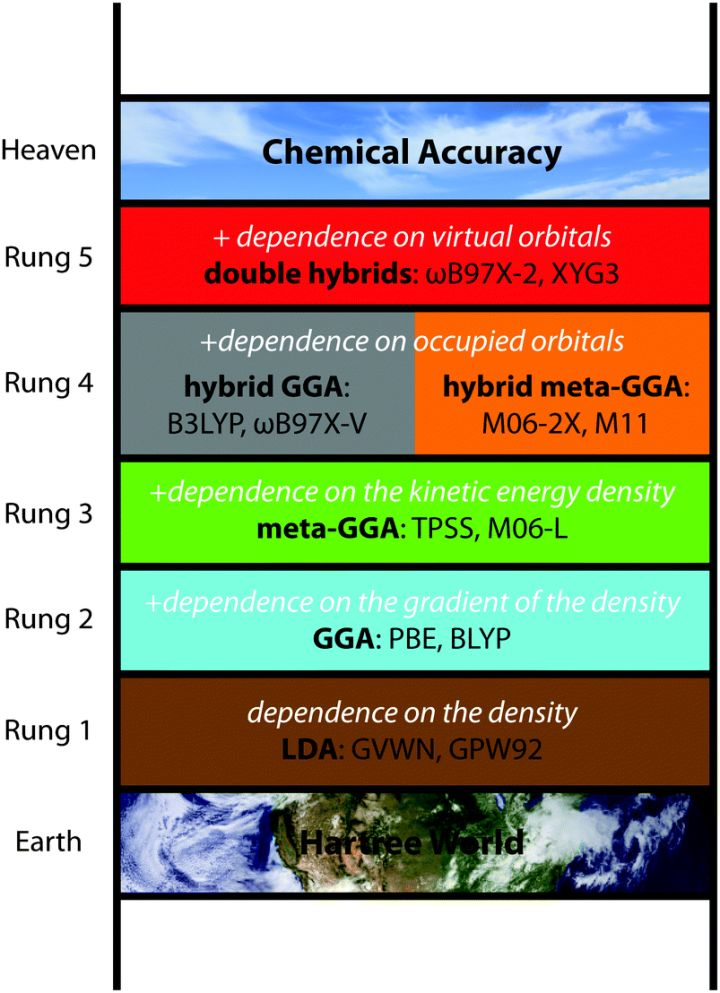
\includegraphics[width=0.3\textwidth]{./images/JoacbLadder.jpg}
\caption{\label{jacobladder}Jacob's Ladder\cite{luintroduction}}
\end{figure}

The bottom of Figure \ref{jacobladder} is the basic Hartree potential, which is the $V_{H}$ term of K-S equations. Through the bottom to the top, different approximation method would get higher accuracy compared to lower level method. This is an invaluable topic to improve the first principle calculation method. The more advanced method could make the calculation closer to the real chemical accuracy, which is also what the future research would focus on. 

\section{Computational Projects}

\subsection{Projects Overview}

With the development of first-principle calculation, the corresponded theory has been transferred into the computational projects based on the programming and computing technique. In order to utilize the first principle theory on the computation simulation, databases, simulation package and pre/post processing tools are always needed to make a complete simulation research.\\
\par Nowadays the famous computational databases include Materials Project\cite{jain2013commentary}, AFLOW\cite{curtarolo2012aflow} and The Open Quantum Materials Database\cite{saal2013materials}. The famous simulation package includes The Vienna Ab initio simulation package (VASP)\cite{hafner2008ab}\cite{kresse1996software} and Abinit\cite{gonze2005brief}. The pre/post process tools includes visualization tools and high throughout calculation library or API, among which the famous one is Pymatgen\cite{ong2013python}. In addition, the useful visualization tools include VESTA\cite{momma2011vesta} and OVITO\cite{stukowski2009visualization}.

\subsection{Sample Computation}

Strontium titanate is a widely used dielectric materials for high-voltage capacitors. Its special superconductivity at high electron densities (doped) below 0.35 K makes itself the first insulator and oxide discovered to behave the superconductivity\cite{koonce1967superconducting}. It is a common phenomena that oxygen vacancies induce free electrons exist in the conduction band of the material\cite{kalabukhov2007effect}. This situation will make the materials become more conductive. In this way, it is valuable to study the oxygen distribution in strontium titanate and further study the vacancy behavior. The structural data (Figure \ref{sto}) for Strontium Titanate is extracted from Materials Project database, which is achieved through API in Pymatgen. Then the generated structural file will be transfered into POSCAR format, which could be used for VASP calculation. The VASP calculation jobs will be submitted to the San Diego Supercomputer Center, which could provide the parallel computing environment and GPU resources. When the computation finished, the result could be utilized by the Python workflow to get the vacancy formation energy data. The Figure \ref{sto-v} shows that the vacancy formation energy at different locations near the grain boundary, through which the most possible vacancy occurrence sites could be found at different layers since the less the formation energy is, the easier the oxygen vacancy can be formed.

\begin{figure}[ht]
\centering
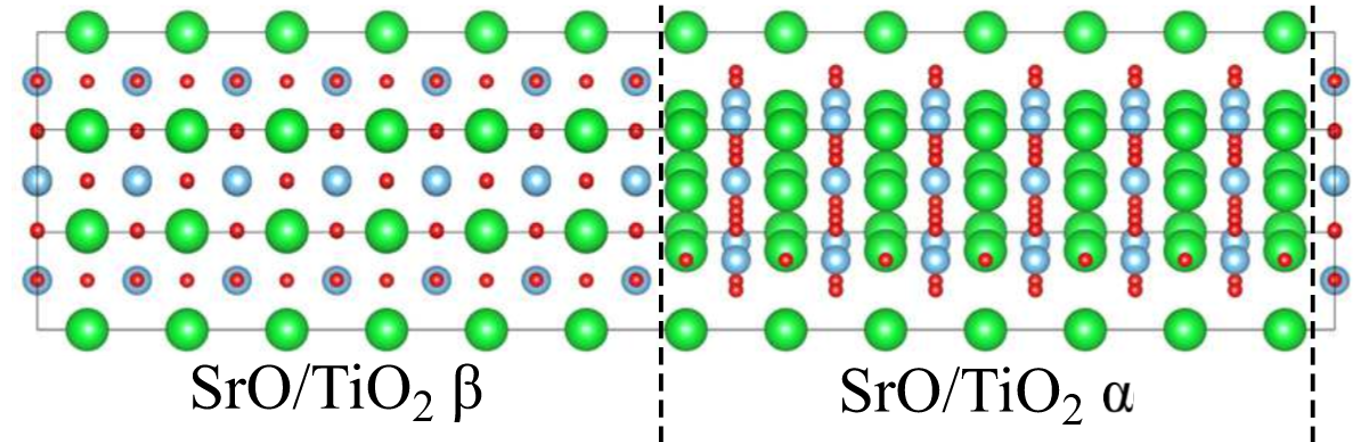
\includegraphics[width=0.4\textwidth]{./images/STO}
\caption{\label{sto}Strontium Titanate with grain boundary\cite{behtash2018oxygen}}
\end{figure}

\begin{figure}[ht]
\centering
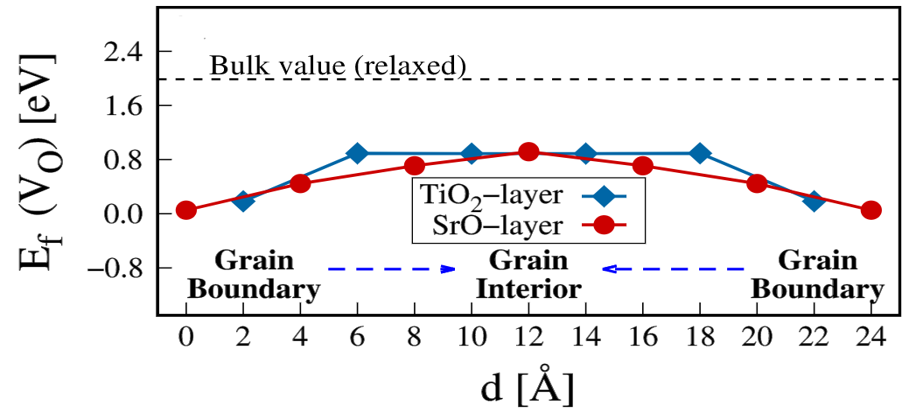
\includegraphics[width=0.4\textwidth]{./images/STO-vacancy}
\caption{\label{sto-v}Oxygen Vacancy Formation Energy At Different Positions\cite{behtash2018oxygen}}
\end{figure}

\section{Conclusions}
First principle is a useful computation method that could be a great help for scientific research acceleration. The most difficult part in this theory is still being improved from mathematical aspects. The development of computing technique could give effective support for the massive computation. In the future, the computational research approach will attract more attention and become more useful for the research projects.

\bibliographystyle{abbrv}
\bibliography{ref}

\end{document}
